\chapter{Resultados y Análisis}

Una vez realizados los experimentos con el algoritmo de agrupamiento X-Means, se presentan los resultados en diferentes figuras y tablas. Primero se encuentran los resultados conseguidos al ejecutar el algoritmo con los atributos de las tablas \ref{tab:atributos_establecimientos} y \ref{tab:atributos_matriculas}, para ver cuales atributos son los mas importantes. Luego se presentan los resultados al comparar el mejor resultado de la etapa anterior con el resultado que se obtiene al agregarle las variables de relación establecimiento-matrícula.

\section{Resultados obtenidos}

La tabla \ref{tab:cl_estab} muestra los resultados al ejecutar X-Means sobre la base de datos de establecimientos en 3 diferentes ocasiones, diferenciándose por la cantidad de atributos que se utilizan. Una con todos los atributos, una con los de importancia alta y media, y finalmente una solo con los atributos de importancia alta.

Las siglas de los clústers de establecimientos sin considerar los atributos de relación establecimientos-matrícula (tablas \ref{tab:cl_estab}, \ref{tab:cl_atr_estab} y \ref{tab:cl_depe_estab}) corresponden a:

\begin{itemize}
    \item BCBM: Bajo Costo Baja Matricula (menor a 390 alumnos).
    \item BCAM: Bajo Costo Alta Matricula (sobre 700 alumnos).
    \item MCAM: Medio Costo Alta Matricula (sobre 700 alumnos).
    \item ACMM: Alto Costo Media Matrícula (entre 391 y 700 alumnos).
\end{itemize}

\begin{table}[H]
\centering
\caption{Clústers de establecimientos variando la cantidad de atributos (por grupos de importancia).}
\label{tab:cl_estab}
\begin{tabular}{|c|c|c|c|c|}
\hline
\textbf{Atributos} & \textbf{BCBM} & \textbf{BCAM} & \textbf{MCAM} & \textbf{ACMM}   \\ \hline
Todos & 959 & 826 & 247 & 36 \\ \hline
Alta + Media & 959 & 540 & 311 & 258 \\ \hline
Alta & 977 & 524 & 308 & 259\\ \hline
\end{tabular}
\end{table}

La tabla \ref{tab:cl_atr_estab} muestra los resultados obtenidos al ejecutar X-Means en los atributos de la base de datos de establecimientos (tabla \ref{tab:atributos_establecimientos}) con importancia alta.

\begin{table}[H]
\centering
\caption{Comparativa de clústers de establecimientos por atributo.}
\label{tab:cl_atr_estab}
\resizebox{\textwidth}{!}{\begin{tabular}{|l|l|l|l|l|}
\hline
& \textbf{BCBM} & \textbf{BCAM} & \textbf{MCAM} & \textbf{ACMM} \\ \hline
\textbf{Dependencia}                    & P.Subvencionado / Municipal & \begin{tabular}[c]{@{}l@{}}P. Subvencionado / Municipal / \\ Corp. Adm. Deleagada\end{tabular} & P. Subvencionado   & P. Pagado        \\ \hline
\textbf{Educación}               & Básica / Media              & Media / Completa                                                                               & Media / Completa   & Completa         \\ \hline
\textbf{Matrícula}               & Gratuita / Menor a \$25.000 & Gratuita / Menor a \$25.000                                                                    & Menor a \$10.000   & Mayor a \$50.000 \\ \hline
\textbf{Mensualidad}             & Gratuita / Menor a \$25.000 & Gratuita / Menor a \$25.000                                                                    & $25.000 - $100.000 & Mayor a \$50.000 \\ \hline
\textbf{Convenio SEP}            & Si                          & Si                                                                                             & No                 & No               \\ \hline
\textbf{Prom. matrículas}        & 383                         & 781                                                                                            & 905                & 686              \\ \hline
\textbf{Prom. alumnos por curso} & 26                          & 30                                                                                             & 32                 & 21               \\ \hline
\textbf{Prom. de becas}          & 19                          & 59                                                                                             & 91                 & 8                \\ \hline
\end{tabular}}
\end{table}

\begin{table}[H]
\centering
\caption{Clústers de establecimientos (tabla \ref{tab:cl_atr_estab}) según su dependencia.}
\label{tab:cl_depe_estab}
\begin{tabular}{|c|c|c|c|c|}
\hline
\textbf{Clúster} & \textbf{Municipal} & \textbf{P. Subvencionado} & \textbf{P. Pagado} & \textbf{Corp. Admin. Del.}   \\ \hline
BCBM & 485 & 491 & 1 & 0 \\ \hline
BCAM & 173 & 318 & 0 & 33 \\ \hline
MCAM & 3 & 303 & 2 & 0 \\ \hline
ACMM & 0 & 1 & 258 & 0 \\ \hline
\end{tabular}
\end{table}

En la tabla \ref{tab:cl_atr_estab_rel} se encuentran los resultados que se obtuvieron al ejecutar el algoritmo de agrupamiento en la base de datos conformada por los atributos de importancia alta de la tabla \ref{tab:atributos_establecimientos} y los atributos de relación establecimiento-matrícula de la tabla \ref{tab:atributos_relacion_establecimientos}.

Las siglas utilizadas para los clústers de establecimientos considerando los atributos de relación establecimientos-matrícula (tablas \ref{tab:cl_atr_estab_rel}, \ref{tab:cl_depe_estab_rel} y \ref{tab:cl_estab_sobre_edad}) corresponden a:
\begin{itemize}
    \item BCBMCD: Bajo Costo Baja Matricula (menor a 390 alumnos) Corta Distancia (menor a 4 km).
    \item BCAMMD: Bajo Costo Alta Matricula (sobre 700 alumnos) Media Distancia (entre 4 y 8 km).
    \item MCAMMD: Medio Costo Alta Matricula (sobre 700 alumnos) Media Distancia (entre 4 y 8 km).
    \item ACMMLD: Alto Costo Media Matrícula (entre 391 y 700 alumnos) Larga Distancia (sobre 8 km).
\end{itemize}

\begin{table}[H]
\centering
\caption{Comparativa de clústers de establecimientos por atributo, incluyendo los de relación establecimiento-matrícula.}
\label{tab:cl_atr_estab_rel}
\resizebox{\textwidth}{!}{\begin{tabular}{|l|l|l|l|l|}
\hline
& \textbf{BCBMPD} & \textbf{BCAMMD} & \textbf{MCAMMD} & \textbf{ACMMLD} \\ \hline
\textbf{Dependencia}                                                                  & P. Subvencionado / Municipal & \begin{tabular}[c]{@{}l@{}}P. Subvencionados / Municipales /\\ Corp. Adm. Delegada\end{tabular} & P. Subvencionado   & P. Pagado        \\ \hline
\textbf{Educación}                                                                    & Básica                       & Media / Completa                                                                                & Media / Completa   & Completa         \\ \hline
\textbf{Matrícula}                                                                    & Gratuita                     & Gratuita / Menor a \$25.000                                                                     & Menor a \$10.000   & Mayor a \$50.000 \\ \hline
\textbf{Mensualidad}                                                                  & Gratuita / Menor a \$25.000  & Gratuita / Menor a \$25.000                                                                     & $25.000 - $100.000 & Mayor a \$50.000 \\ \hline
\textbf{Convenio SEP}                                                                 & Si                           & Si                                                                                              & No                 & No               \\ \hline
\textbf{Prom. matrículas}                                                             & 383                          & 781                                                                                             & 895                & 686              \\ \hline
\textbf{Prom. alumnos por curso}                                                      & 26                           & 30                                                                                              & 32                 & 21               \\ \hline
\textbf{Prom. de becas}                                                               & 19                           & 58                                                                                              & 91                 & 8                \\ \hline
\textbf{IDE}                                                                          & 0,5 - 1                      & -0,5 - 0                                                                                        & 0 - 1,5            & 1 - 1,5          \\ \hline
\begin{tabular}[c]{@{}l@{}}\textbf{Distancia}\\ \textbf{Establecimiento - Hogar}\end{tabular} & 2,960 km                     & 5,204 km                                                                                        & 5,207 km           & 9,761            \\ \hline
\textbf{Sobre edad promedio}                                                                   & 0,524                        & 0,488                                                                                           & 0,297              & 0,488            \\ \hline
\end{tabular}}
\end{table}

\begin{table}[H]
\centering
\caption{Clústers de establecimientos (tabla \ref{tab:cl_atr_estab_rel}) según su dependencia.}
\label{tab:cl_depe_estab_rel}
\begin{tabular}{|c|c|c|c|c|}
\hline
\textbf{Clúster} & \textbf{Municipal} & \textbf{P. Subvencionado} & \textbf{P. Pagado} & \textbf{Corp. Admin. Del.}   \\ \hline
BCBMPD & 485 & 489 & 1 & 0 \\ \hline
BCAMMD & 173 & 307 & 0 & 33 \\ \hline
MCAMMD & 3 & 316 & 2 & 0 \\ \hline
ACMMLD & 0 & 1 & 258 & 0 \\ \hline
\end{tabular}
\end{table}

\begin{table}[H]
\centering
\caption{Detalle de la sobre edad en los clústers de establecimientos. }
\label{tab:cl_estab_sobre_edad}
\begin{tabular}{|l|c|c|c|c|c|}
\hline
                & \textbf{\% del total} & \textbf{\% 1 año\footnotemark} & \textbf{\% 2 años\footnotemark[\value{footnote}]\footnotemark[\value{footnote}]} & \textbf{\% 3 años\footnotemark[\value{footnote}]} & \textbf{\% 4 años\footnotemark[\value{footnote}]} \\ \hline
\textbf{BCBMPD} & 31                    & 74,8              & 18,9               & 5,2                & 1,1                \\ \hline
\textbf{BCAMMD} & 32,9                  & 75,1              & 20,5               & 3,9                & 0,5                \\ \hline
\textbf{MCAMMD} & 24                    & 85,3              & 13                 & 1,6                & 0,1                \\ \hline
\textbf{ACMMLD} & 38,1                  & 94,9              & 4,6                & 0,4                & 0,1                \\ \hline
\end{tabular}
\end{table}

\footnotetext{Porcentajes en base al total de alumnos con sobre edad mayor o igual a 1.}

Las siguientes tablas, y de manera similar a lo descrito anteriormente para los establecimientos, muestran los resultados obtenidos usando los datos de las matrículas. En la tabla \ref{tab:cl_mat} se muestran los resultados con los datos de la tabla \ref{tab:atributos_matriculas} en 3 diferentes versiones, según la importancia del atributo. La primera con todos los atributos, luego solo con los de alta y media, y finalmente solo los de alta importancia.

Las siglas utilizadas para los clústers de matrículas sin atributos de relación (tablas \ref{tab:cl_mat}, \ref{tab:cl_atr_mat} y \ref{tab:cl_mat_sobre_edad}) corresponden a:

\begin{itemize}
    \item MCB: Mujeres Con Beneficio.
    \item HCB: Hombres Con Beneficio.
    \item MSB: Mujeres Sin Beneficio.
    \item HSB: Hombres Sin Beneficio.
\end{itemize}

\begin{table}[H]
\centering
\caption{Clústers de matrículas variando la cantidad de atributos (por grupos de importancia).}
\label{tab:cl_mat}
\begin{tabular}{|c|c|c|c|c|}
\hline
\textbf{Atributos} & \textbf{MCB} & \textbf{HCB} & \textbf{MSB} & \textbf{HSB}   \\ \hline
Todos & 551932 & 442048 & 40803 & 13585 \\ \hline
Alta + Media & 551932 & 442048 & 34088 & 20300 \\ \hline
Alta & 286089 & 300007 & 230486 & 231786 \\ \hline
\end{tabular}
\end{table}

En las tablas \ref{tab:cl_atr_mat} y \ref{tab:cl_atr_mat_rel} se muestran primero los resultados obtenidos al utilizar los atributos de alta importancia de la tabla \ref{tab:atributos_matriculas} y luego los que se obtienen al incluir los atributos de relación de la tabla \ref{tab:atributos_relacion_matriculas}.

\begin{table}[H]
\centering
\caption{Comparativa de clústers de matrículas por atributo.}
\label{tab:cl_atr_mat}
\resizebox{\textwidth}{!}{\begin{tabular}{|l|l|l|l|l|}
\hline
& \textbf{MCB} & \textbf{HCB} & \textbf{MSB} & \textbf{HSB} \\ \hline
\textbf{Género}           & Femenino                                                                                                         & Masculino                                                                                                        & Femenino & Masculino \\ \hline
\textbf{Beneficiario SEP} & Si                                                                                                               & Si                                                                                                               & No       & No        \\ \hline
\textbf{Criterio SEP}     & \begin{tabular}[c]{@{}l@{}}Pertenece a Chile solidario / \\ Puntaje de ficha de protección\\ social\end{tabular} & \begin{tabular}[c]{@{}l@{}}Pertenece a Chile solidario / \\ Puntaje de ficha de protección\\ social\end{tabular} &          &           \\ \hline
\textbf{Sobre edad}       & 0,364                                                                                                            & 0,488                                                                                                            & 0,284    & 0,365     \\ \hline
\end{tabular}}
\end{table}


\begin{table}[H]
\centering
\caption{Detalle de la sobre edad en los clústers de matrículas.}
\label{tab:cl_mat_sobre_edad}
\begin{tabular}{|l|c|c|c|c|c|}
\hline
             & \textbf{\% del total} & \textbf{\% 1 año\footnotemark} & \textbf{\% 2 años\footnotemark[\value{footnote}]} & \textbf{\% 3 años\footnotemark[\value{footnote}]} & \textbf{\% 4 años\footnotemark[\value{footnote}]} \\ \hline
\textbf{MCB} & 28,5                  & 76,9              & 18,5               & 4                  & 0,6                \\ \hline
\textbf{HCB} & 36,4                  & 72,5              & 21,5               & 5,1                & 0,9                \\ \hline
\textbf{MSB} & 25,7                  & 90.2              & 8,7                & 1                  & 0,1                \\ \hline
\textbf{HSB} & 32                    & 87,3              & 11,1               & 1,5                & 0,1                \\ \hline
\end{tabular}
\end{table}

\footnotetext{Porcentajes en base al total de matrículas con sobre edad mayor o igual a 1.}

Las siglas utilizadas para los clústers de matrículas, incluyendo los atributos de relación, (tablas \ref{tab:cl_atr_mat_rel} y \ref{tab:cl_mat_rel_sobre_edad}) corresponden a:

\begin{itemize}
    \item MCBBC: Mujeres Con Beneficio Bajo Costo.
    \item HCBBC: Hombres Con Beneficio Bajo Costo.
    \item MiSBMC: Mixto Sin Beneficio Medio Costo.
    \item MiSBAC: Mixto Sin Beneficio Alto Costo.
\end{itemize}

\begin{table}[H]
\centering
\caption{Comparativa de clústers de matrículas por atributo, incluyendo los de relación  establecimiento-matrícula.}
\label{tab:cl_atr_mat_rel}
\resizebox{\textwidth}{!}{\begin{tabular}{|l|l|l|l|l|}
\hline
& \textbf{MCBBC} & \textbf{HCBBC} & \textbf{MiSBMC} & \textbf{MiSBAC} \\ \hline
\textbf{Género}                                                                      & Femenino                                                                                                        & Masculino                                                                                                       & Femenino / Masculino & Femenino / Masculino \\ \hline
\textbf{Beneficiario SE}P                                                            & Si                                                                                                              & Si                                                                                                              & No                   & No                   \\ \hline
\textbf{Criterio SEP}                                                                & \begin{tabular}[c]{@{}l@{}}Pertenece a Chile solidario /\\ Puntaje de ficha de protección\\ social\end{tabular} & \begin{tabular}[c]{@{}l@{}}Pertenece a Chile solidario /\\ Puntaje de ficha de protección\\ social\end{tabular} &                      &                      \\ \hline
\textbf{Sobre edad}                                                                  & 0,370                                                                                                           & 0,492                                                                                                           & 0,270                & 0,401                \\ \hline
\textbf{Matrícula que paga}                                                          & Gratuita                                                                                                        & Gratuita                                                                                                        & Gratuita             & Mayor a \$100.000    \\ \hline
\textbf{Mensualidad que paga}                                                        & Gratuita                                                                                                        & Gratuita                                                                                                        & $10.000 - $100.000   & Mayor a \$100.000    \\ \hline
\begin{tabular}[c]{@{}l@{}}\textbf{Distancia}\\ \textbf{Establecimiento - Hogar}\end{tabular} & 4,711 km                                                                                                        & 4,939 km                                                                                                        & 5,912 km             & 4,911 km             \\ \hline
\end{tabular}}
\end{table}

\begin{table}[H]
\centering
\caption{Detalle de la sobre edad en los clústers de matrículas, incluyendo atributos de relación.}
\label{tab:cl_mat_rel_sobre_edad}
\begin{tabular}{|l|c|c|c|c|c|}
\hline
                & \textbf{\% del total} & \textbf{\% 1 año\footnotemark} & \textbf{\% 2 años\footnotemark[\value{footnote}]} & \textbf{\% 3 años\footnotemark[\value{footnote}]} & \textbf{\% 4 años\footnotemark[\value{footnote}]} \\ \hline
\textbf{MCBBC}  & 28,9                  & 76,7              & 18,7               & 3,9                & 0,7                \\ \hline
\textbf{HCBBC}  & 36,7                  & 72,4              & 21,6               & 5,1                & 0,9                \\ \hline
\textbf{MiSBMC} & 23,4                  & 85,9              & 12,4               & 1,6                & 0,1                \\ \hline
\textbf{MiSBAC} & 38,1                  & 94,9              & 4,6                & 0,4                & 0,1                \\ \hline
\end{tabular}
\end{table}

\footnotetext{Porcentajes en base al total de matrículas con sobre edad mayor o igual a 1.}

\section{Análisis de los resultados}

En esta sección se analizan los diferentes resultados obtenidos y presentados anteriormente, comenzando con el análisis para los establecimientos y seguido por el de las matrículas.

Lo primero que se aprecia en la tabla \ref{tab:cl_estab}, es que para las 3 versiones el clúster BCBM agrupa casi un 50\% del total de los colegios, en donde además en la segunda y tercera versión el resto de los clústers presentan una cardinalidad similar. Esto demuestra que en este caso incluir variables consideradas de importancia media y baja no generan un gran impacto en el resultado final.

Teniendo en cuenta lo anterior, y de que por tratarse de un aprendizaje no supervisado es difícil establecer una medida de eficiencia, se consideró la tercera versión para el resto del estudio. Es decir, se tomará la versión en la cual solo se utilizaron los atributos clasificados como de alta importancia. Además se debe considerar que al ejecutar el algoritmo con menos variables el tiempo de ejecución es menor.

A partir de los resultados obtenidos para los establecimientos y de las figuras generadas con estos (figuras \ref{fig:radar_estab} y \ref{fig:radar_estab_rel}), podemos ver que al realizar una comparación entre ambas ejecuciones del algoritmo (sin y con atributos de relación) no se generan grandes cambios en los clústers, pero si aumenta el nivel de información y detalle de cada uno de ellos, incorporando nuevas características distintivas. Es por esto que el análisis se centrará en dichos resultados.

\begin{figure}[hc]
    \centering
    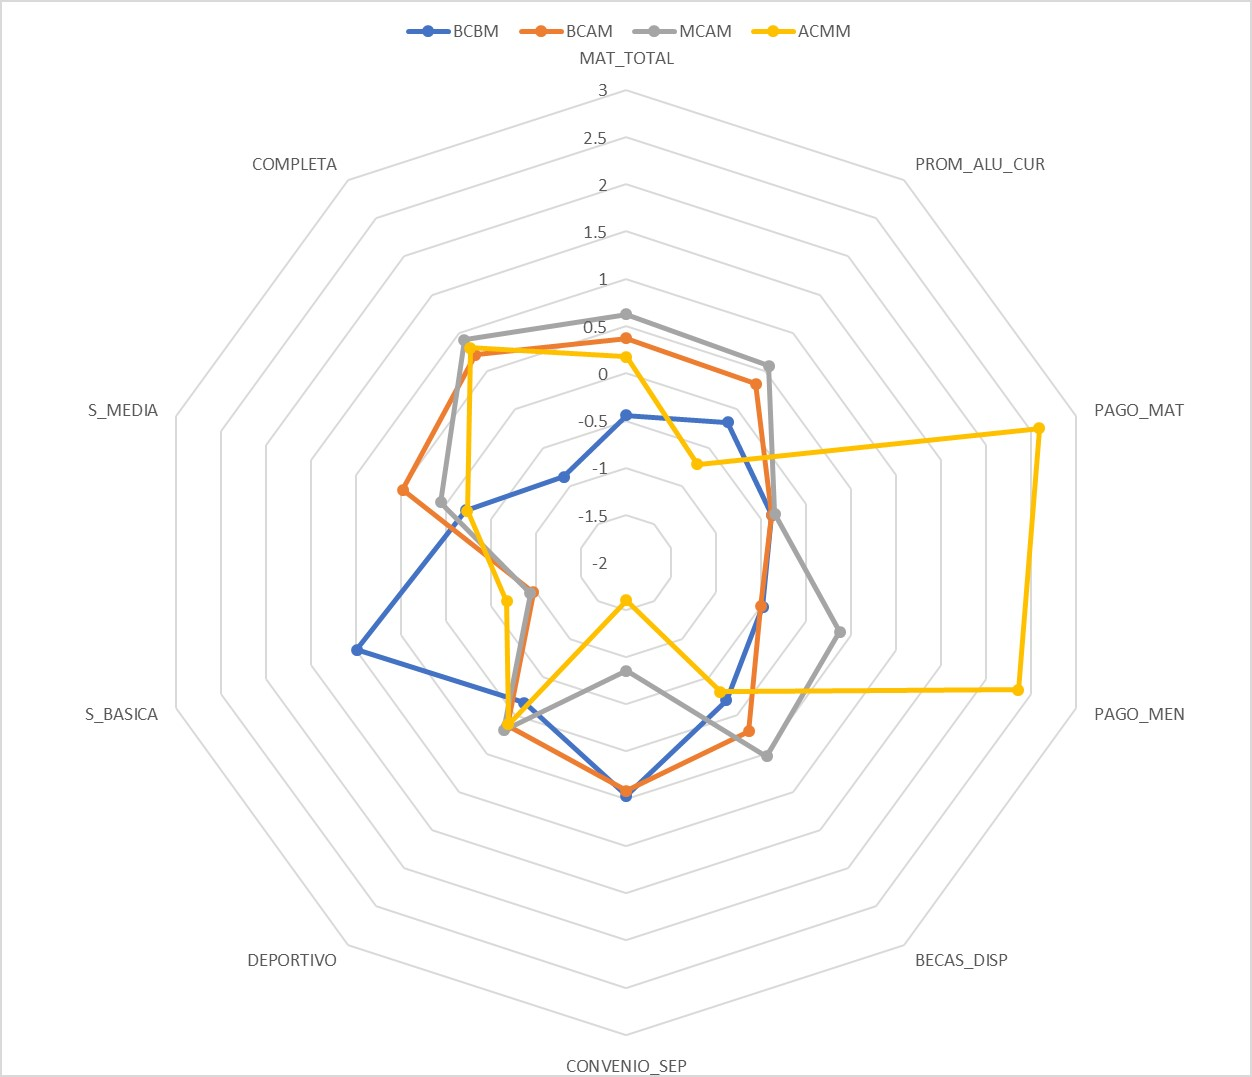
\includegraphics[width=0.66\textwidth]{images/radar_chart_establecimientos_sin.jpg}
    \caption{Promedios de atributos normalizados para establecimientos de la Región Metropolitana.}
    \label{fig:radar_estab}
\end{figure}

\begin{figure}[hc]
    \centering
    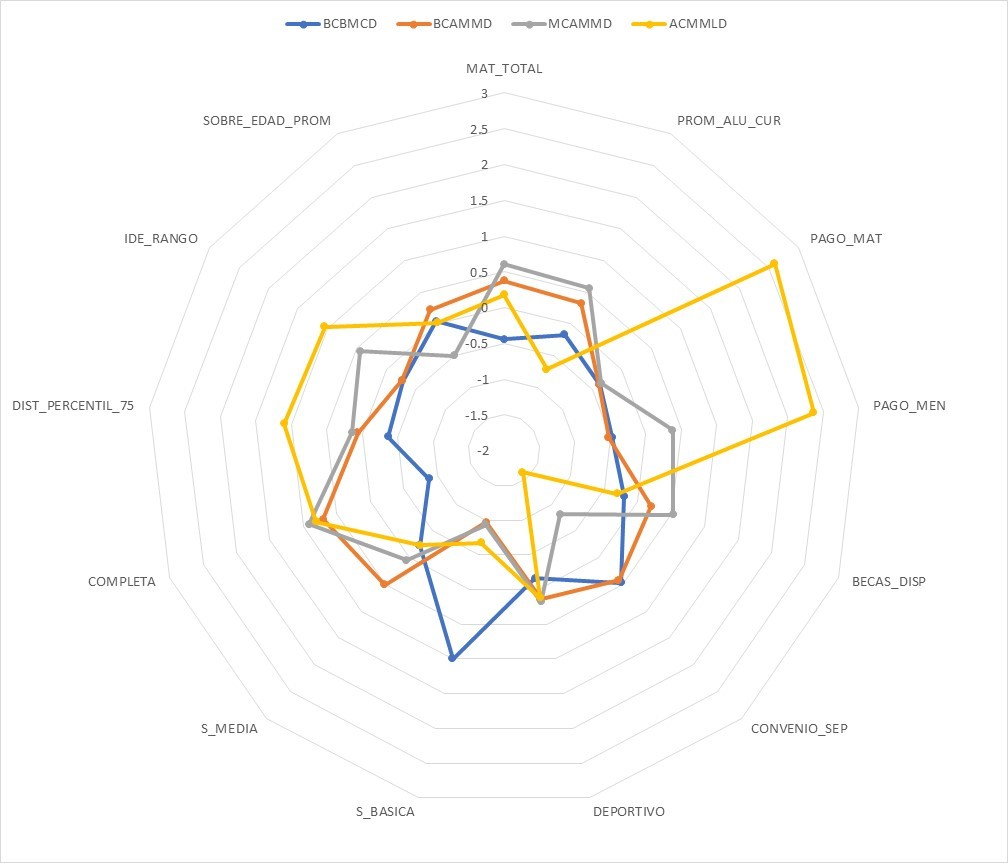
\includegraphics[width=0.66\textwidth]{images/radar_chart_establecimientos_con.jpg}
    \caption{Promedios de atributos normalizados de establecimientos con atributos relacionales (tabla \ref{tab:atributos_relacion_establecimientos}) de la Región Metropolitana.}
    \label{fig:radar_estab_rel}
\end{figure}

Los primeros dos clústers son colegios gratuitos o baratos con un IDE bajo que se diferencian entre ellos principalmente por el nivel de educación que imparten, en el primero predominan los de enseñanza básica y en el segundo establecimientos que imparten educación media o completa. El tercer y cuarto clúster se diferencia de los otros dos por tener un nivel de copago e IDE superiores, donde en el tercero se tienen valores medios y en el cuarto valores elevados. Por otro lado, al analizar la distancia que separa a los establecimientos de sus estudiantes, se aprecia notoriamente que el desplazamiento crece al aumentar el nivel del copago. Es decir, las familias que más pagan están dispuestas a desplazarse distancias mayores para llegar al establecimiento en comparación a familias que optan por colegios gratuitos o de bajo costo. Finalmente otro punto interesante de analizar es la sobre edad, que en el caso de los colegios más caros se concentra con un 95\% en un año de sobre edad. En el resto de los clústers el valor fluctúa entre un 75\% y 85\%, y el resto de distribuye de 2 a 4 años de sobre edad.

Para el caso de las matrículas lo primero que se debe analizar es la tabla \ref{tab:cl_mat}, en donde se aprecian los resultados de las 3 ejecuciones con los diferentes atributos, agrupados por su nivel de importancia. Se puede ver que las primeras dos ejecuciones generan clústers de cardinalidad muy similares, diferenciándose claramente con el tercer resultado, el cual presenta clústers de tamaños similares. La diferencia se en que los clústers de la última ejecución poseen atributos que describen de mejor manera los grupos, los cuales se van perdiendo al ir añadiendo atributos adicionales. 

Además de lo ya mencionado, es importante tener en cuenta que agregar más atributos a una base de datos de un total de 1.500.000 registros aproximadamente, provocará que el tiempo requerido para su ejecución aumenta significativamente. Por lo tanto, se analizarán más a fondo los resultados de la tercera ejecución y se utilizará para comparar con los resultados que se obtienen al agregar los atributos de relación.

\begin{figure}[hc]
    \centering
    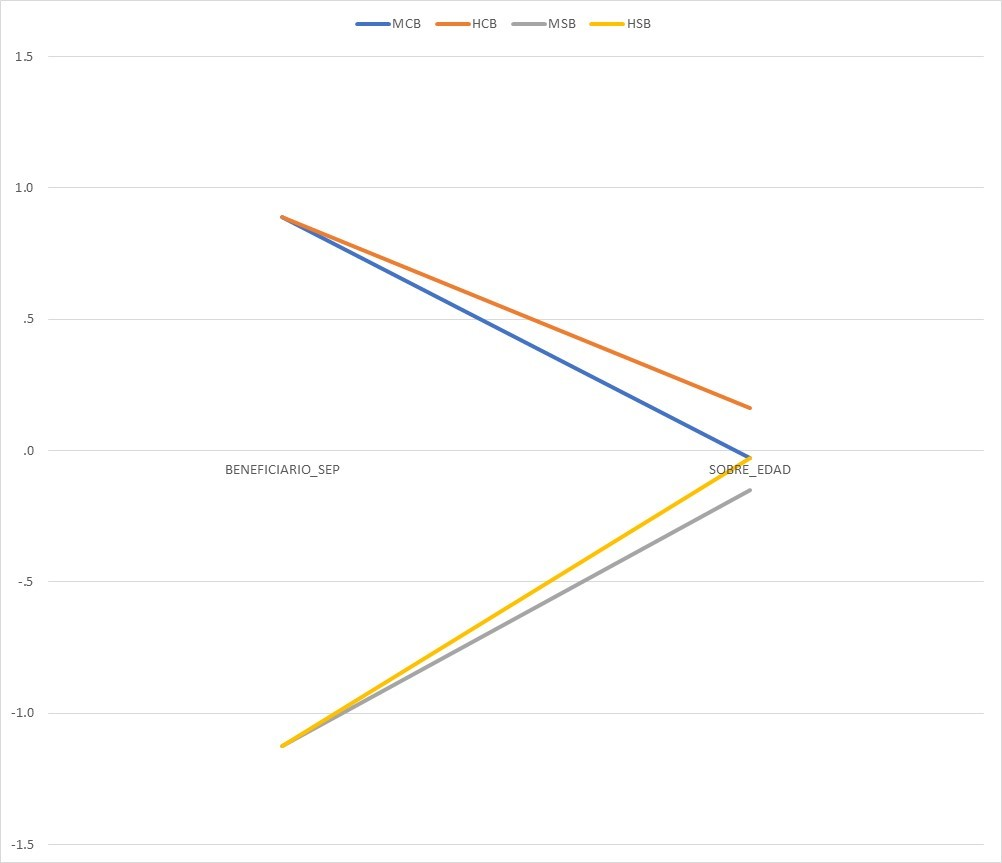
\includegraphics[width=0.66\textwidth]{images/chart_matriculas_sin.jpg}
    \caption{Promedio de atributos normalizados de matrículas de la Región Metropolitana.}
    \label{fig:chart_mat}
\end{figure}

\begin{figure}[hc]
    \centering
    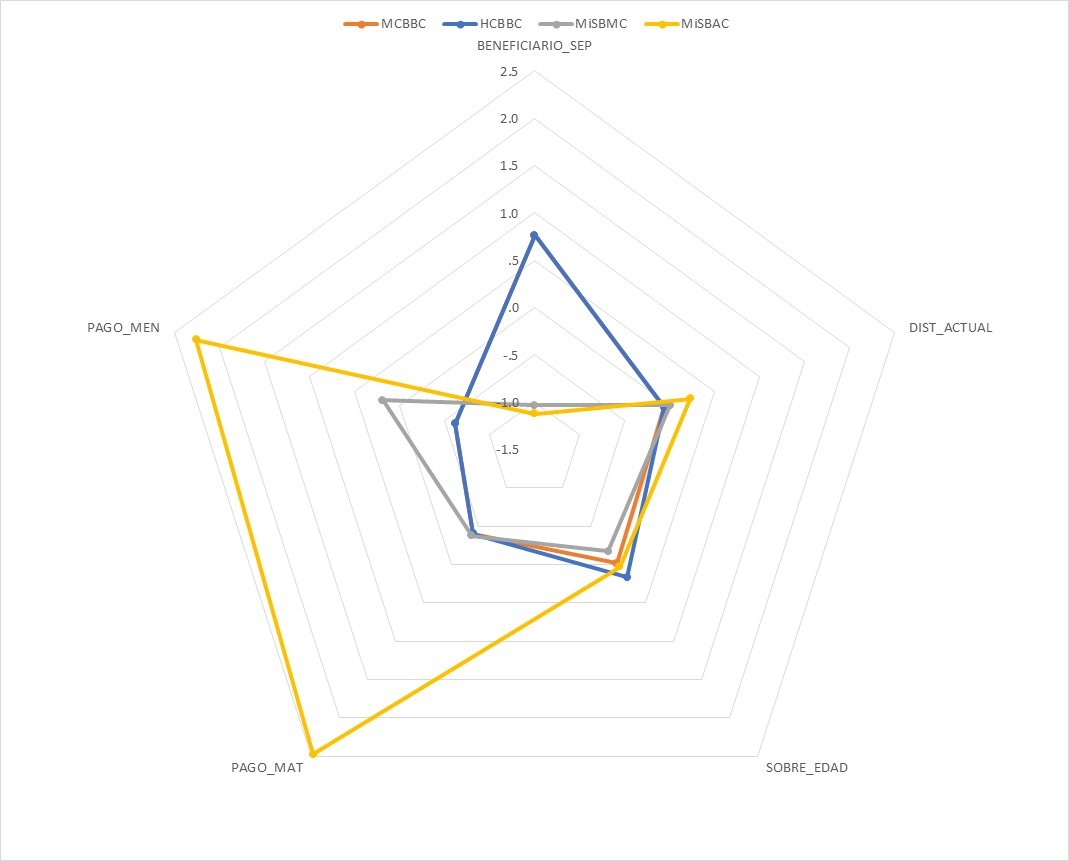
\includegraphics[width=0.66\textwidth]{images/radar_chart_matriculas_con.jpg}
    \caption{Promedio de atributos normalizados de matrículas con atributos relacionales (tabla \ref{tab:atributos_relacion_matriculas}) de la Región Metropolitana.}
    \label{fig:radar_mat_rel}
\end{figure}

Lo siguiente a analizar son las diferentes características de los clústers obtenidos para las matrículas y compararlos con los que se obtienen cuando se agregan los atributos de relación. Para facilitar la comparación entre clústers se generaron las figuras \ref{fig:chart_mat} y \ref{fig:radar_mat_rel}.